\subsection{RSS3 \glsfmtfull{GI}}
\label{subsec:GI}

{
    \begin{figure}[tb!]
        \centering
        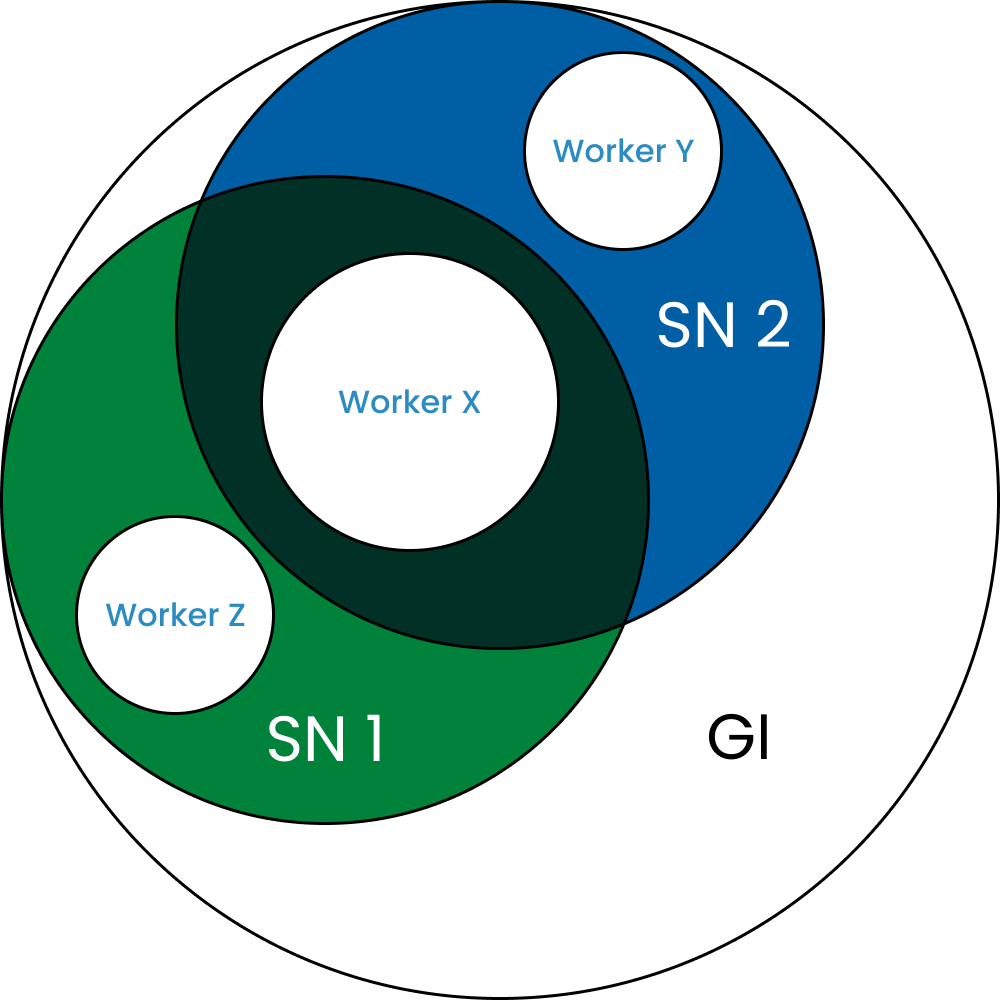
\includegraphics[width=0.7\columnwidth]{figures/GI.png}
        \caption{A Venn diagram illustrating the relationship between the worker, the \glsfmtlong{Node}, and the \glsfmtlong{GI}.}
        \label{fig:GI}
    \end{figure}
}

\glspl{GI} are responsible for facilitating coordination among \glspl{Node} and engaging with the \gls{VSL} and perform critical duties to ensure the \gls{DSL} is robust and reliable.

Given the importance of the \glspl{GI} to the Network, their operation is subject to a set of stringent requirements imposed by the Network.

{
    \begin{figure}[tb!]
        \centering
        \includegraphics[width=1\columnwidth]{figures/GI-components.png}
        \caption{The core components of \gls{GI}.}
        \label{fig:GI-components}
    \end{figure}
}

\subsubsection{Router}
The router of \gls{GI} ensures requests are routed and served with high performance and minimal latency.
The unique architecture of the \gls{DSL} demands \gls{GI} to be equipped with more computational capabilities to work out the optimal route for processing incoming requests. A request often retrieves \glsfmtlong{OI} from a single \gls{Node} and frequently from a group of \glspl{Node} simultaneously.

\subsubsection{Broadcaster and Enforcer}
The broadcaster and enforcer of \gls{GI} act as supervisors for \glspl{Node} to ensure the quality of service. The broadcaster constantly monitors all \glspl{Node}' status for irregular behaviors. With the \gls{DSL} being a permissionless Sublayer, the quality needs to be maintained strictly to ensure \glsfmtlong{R3N}'s robustness and reliability.
The enforcer works with the broadcaster and router to maintain a record of demotion and slashing, and slash a \gls{Node} if it fails to meet the requirements.

\subsubsection{Settler}
The settler of \gls{GI} initiates submissions of work records of \glspl{Node} to the \gls{VSL}, and the settlement contract will verify and distribute network rewards.

\subsubsection{Payment Processor}
The payment processor (works together with the settler) ensures that requests fees collected are correctly distributed to the corresponding Nodes and creators.
Additionally, the payment processor works out the Network's average tax rate and updates the settlement contract on the \gls{VSL}.

\subsubsection{Indexer}
The indexer is responsible for structuring activities that take place on the entire Network, and supplying the information via network transparency API.

\subsection{Reliability Score}

A \gls{GI} routes requests to \glspl{Node} based on their information coverage and a \gls{RS}.
The calculation of \reliabilityScore\ is based on a range of factors, including but not limited to the \gls{Node}'s uptime, work, slash records, operation deposit, and staking/trust pool size.
\glspl{Node} with a higher \reliabilityScore\ have an increased likelihood of receiving requests.
